\documentclass[12pt,prb,aps,epsf]{article}
\usepackage[utf8]{inputenc}
\usepackage{amsmath}
\usepackage{amsfonts}
\usepackage{amssymb}
\usepackage{graphicx} 
\usepackage{latexsym} 
\usepackage[toc,page]{appendix}
%\usepackage{listings}
\usepackage{xcolor}
\usepackage{soul}
\usepackage[T1]{fontenc}
\usepackage{amsthm}
\usepackage{mathtools}
\usepackage{setspace}
\usepackage{array,multirow,makecell}
\usepackage{geometry}
\usepackage{textcomp}
\usepackage{float}
\usepackage{cancel}
\usepackage{here}
\usepackage{titlesec}
\usepackage{bbold}

\geometry{hmargin=2cm,vmargin=2cm}

\begin{document}
	
	\title{MP 32 Oscillateurs couplés}
	\author{Naïmo Davier}
	\date{Agrégation 2019}
	
	\maketitle
	
	\tableofcontents
	
	\pagebreak
	

\section{Deux oscillateurs identiques couplés}	
\subsection{LC couplés via une capacité}	
	On regarde le circuit représenté sur la figure ci dessous
\begin{figure}[h]
\centering 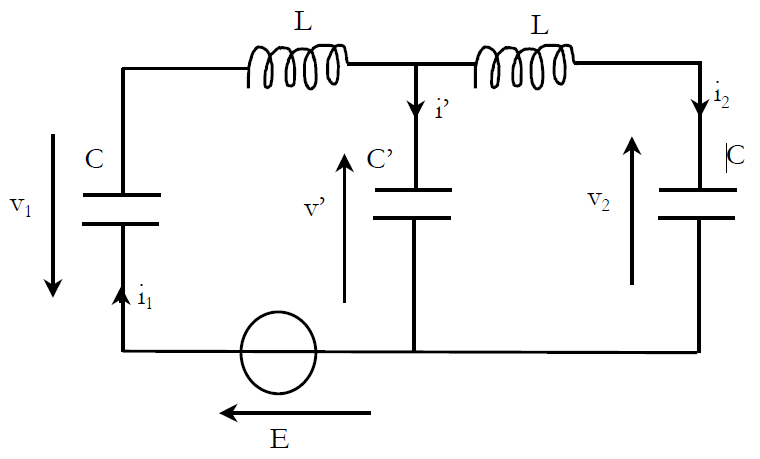
\includegraphics[width=10cm]{RLCcouples}
\end{figure}
	où on va considérer pour plus de généralité une résistance en série de chacune des bobines, et que les capacités et inductances des sous circuits 1 et 2 ne sont pas exactement les mêmes. 
	On a, pour les intensités
	\begin{eqnarray}
	i_1 = C_1\frac{dv_1}{dt}\hspace{1cm} i_2 = C_2\frac{dv_2}{dt}\hspace{1cm} i' = C'\frac{dv'}{dt}
	\end{eqnarray}
	avec, selon la loi des nœuds 
	\begin{eqnarray}
	i_1 = i'+i_2\hspace{0.7cm} \Leftrightarrow \hspace{0.7cm} C_1\frac{dv_1}{dt} = C'\frac{dv'}{dt} + C_2\frac{dv_2}{dt}
	\end{eqnarray}
ce qui conduit à 
	\begin{eqnarray}
	 C'v' = C_1v_1 -C_2v_2
	\end{eqnarray}
en tenant compte du fait qu'à t=0 le circuit n'est pas alimenté.\\
On a alors en appliquant la loi des mailles 
	\begin{eqnarray}
	E = v_1 + L_1\frac{di_1}{dt} + R_1i_1 + v'\\
	0 = -v' + L_2\frac{di_2}{dt} + R_2i_2 + v_2
	\end{eqnarray}
soit 
	\begin{eqnarray}
	E = v_1 + L_1C_1\frac{d^2v_1}{dt^2} + R_1C_1\frac{dv_1}{dt} + \frac{1}{C'}(C_1v_1 -C_2v_2)\\
	0 = -\frac{1}{C'}(C_1v_1 -C_2v_2) + L_2C_2\frac{d^2v_2}{dt^2} + R_2C_2\frac{dv_2}{dt} + v_2
	\end{eqnarray}
	
La suite de la résolution dans le cas de deux oscillateurs identiques et sans dissipation est similaire à celle effectuée dans la partie suivante. On se contentera ici du cas simple où les deux LC (on néglige les résistances) sont les mêmes pour des raisons de simplicité de calcul et d'expression des fréquences propres.

On obtient alors les fréquences propres suivantes 
\begin{eqnarray}
f_s = \frac{1}{2\pi} \frac{1}{\sqrt{LC}}\hspace{1cm}\mathrm{et}\hspace{1cm}f_{as} = \frac{1}{2\pi} \sqrt{\frac{C + 2C'}{LCC'}}
\end{eqnarray}
que l'on va pouvoir identifier expérimentalement de deux manières différentes : soit en regardant $v_1$ et $v_2$ tout en balayant en fréquences avec un GBF délivrant une sinusoïde (permet de montrer que l'un est bien symétrique : tensions en phase, et l'autre antisymétrique : en opposition de phase), soit en envoyant un créneau (de période $T\geq 5l/R$) et en regardant la dérivée de la TF de la réponse indicielle. \\

Si on veut utiliser notre modèle de 2 LC couplés, et ainsi que les 2 fréquences de résonance en tension soit les même pour $v_1$ et $v_2$, on aura intérêt à ne pas ajouter de résistance. En effet on aura alors un bon facteur de qualité, que l'on peut optimiser en prenant $C$ le plus petit possible (puisqu'on a pas le choix pour $L$). Les pics de tension seront alors bien étroits et on pourra ainsi clairement identifier les fréquences des deux modes.\\

On peut maintenant regarder le cas très similaire du point de vue des équation mais d'aspect très différent de deux oscillateurs harmoniques mécaniques couplés.

\subsection{Deux oscillateurs harmoniques mécaniques}
On a deux voiturettes posées sur un support horizontal, liées entre elles et aux extrémités du support par des ressorts de raideur $k$  et $k_2$ (ressort de couplage), ce qui est équivalent au cas de la figure ci dessous.\\
\begin{figure}[h]
	\centering 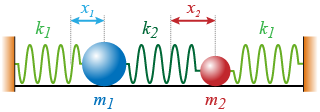
\includegraphics[width=10cm]{oh_couples}
\end{figure}

On voit en appliquant le PFD que l'on a un système de deux équations couplées pour les position des deux masses
\begin{eqnarray}
m\ddot{x}_1 = -kx_1 + k_2(x_2-x_1)\\
m\ddot{x}_2 = -kx_2 - k_2(x_2-x_1)
\end{eqnarray}
que l'on peut réécrire sous forme matricielle 
\begin{eqnarray}
m
\begin{pmatrix}
\ddot{x}_1\\
\ddot{x}_2
\end{pmatrix}
= \begin{pmatrix}
- k - k_2& k\\
k & - k - k_2
\end{pmatrix}
\begin{pmatrix}
x_1\\
x_2
\end{pmatrix}
\end{eqnarray}
équivalent à l'équation type 
\begin{eqnarray}
\ddot{\vec{X}} + \omega_0^2 M\vec{X} = 0
\end{eqnarray}
où
\begin{eqnarray}
M = \begin{pmatrix}
1+\varepsilon & -\varepsilon\\
- \varepsilon & 1+ \varepsilon
\end{pmatrix}
\hspace{1cm}\mathrm{avec}\hspace{1cm} \omega_0^2 = \frac{k_2}{m}\;\;\mathrm{et}\;\; \varepsilon = \frac{k}{k_2}
\end{eqnarray}
La matrice M est diagonalisable, on peut donc la diagonaliser puis effectuer un changement de base afin de se placer dans la base propre du système dans laquelle apparaîtront deux oscillateurs découplés et donc indépendants. Commençons par diagonaliser $M$, pour cela on commence par chercher les valeurs propres en résolvant 
\begin{eqnarray}
\det(M - \lambda \mathbb{1}) = 0\\
\Rightarrow\; (1+\varepsilon-\lambda)^2 &=& \varepsilon^2\\
1 + \varepsilon - \lambda &=& \pm \varepsilon\\
\Rightarrow\;\;\lambda_1 = 1\hspace{1cm}\mathrm{et}\hspace{1cm}\lambda_2 = 1+2\varepsilon
\end{eqnarray}
Ce qui signifie que les deux fréquences propres du systèmes sont $\omega_1 = \omega_0$ et $\omega_2 = (1+2\varepsilon)\omega_0$ où $\omega_0$ est la fréquence propre d'un oscillateur seul (avec un ressort de raideur $k_2$).\\
On peut maintenant chercher les vecteurs propres $\vec{y}_1$ et $\vec{y}_2$ de $M$, commençons par $\vec{y}_1 = \begin{pmatrix}
\alpha_1\\ \beta_1
\end{pmatrix}$ tel que $M\vec{y}_1 = \vec{y}_1$ ce qui équivaut à
\begin{eqnarray}
(1+\varepsilon)\alpha_1 - \varepsilon \beta_1 = \alpha_1\\
\Leftrightarrow \alpha_1 = \beta_1
\end{eqnarray}
On a donc $\vec{y}_1 = \frac{1}{\sqrt{2}}\begin{pmatrix}
1\\ 1
\end{pmatrix}$ ce que l'on peut formuler comme $y_1(t) = \frac{1}{\sqrt{2}}(x_1(t) + x_2(t))$. Si on fait de même pour $\vec{y}_2$ on trouve $y_2(t) = \frac{1}{\sqrt{2}}(x_1(t) - x_2(t))$.\\ Géométriquement le premier mode correspond au cas $y_2(t)=0$ et donc $x_1(t) = x_2(t)$, les deux masses oscillent alors en phase, le ressort central ayant une longueur constamment égale à sa longueur à vide. Le second mode correspond quant à lui à $y_1(t) = 0$ et ainsi $x_1(t) = -x_2(t)$ : mode antisymétrique où les deux masses oscillent en opposition de phase.\\

Expérimentalement on a 
$m_{voiture} = 246,1\pm0,3g$ et $k_1=k_2=k = 6,8 N.m^{-1}$.\\
On en déduit 
\begin{eqnarray}
\omega_{s} = \sqrt{\frac{k}{m}} = 5,256\pm0.006\,rad.s^{-1} \hspace{1cm}&\mathrm{et}&\hspace{1cm}\omega_{as} = \sqrt{\frac{3k}{m}} = 9,10\pm0.01 \,rad.s^{-1}\\
\Rightarrow\;\;f_{s} = 0,837 \,Hz \hspace{1cm}&\mathrm{et}&\hspace{1cm} f_{as} = 1,449\,Hz\\
On\;mesure\;\;f_{s} = 0,807 \,Hz \hspace{1cm}&\mathrm{et}&\hspace{1cm} f_{as} = 1,387\,Hz
\end{eqnarray}
On utilise le logiciel fournit avec les voiturettes pour acquérir la position des voiturettes en fonction du temps. On peut ensuite faire la TF de l'une des vitesses (spectre plus lisible que ceux des postions) pour identifier les différents modes. On peut notamment exciter le mode symétrique ou antisymétrique en prenant les bonnes C.I afin de n'avoir qu'une des deux fréquences propres, ou bien prendre des C.I quelconques et montrer que l'on a une superposition des deux modes via la TF.\\

On a vu qu'on avait une analogie entre mécanique et électronique où l'inductance joue le rôle de masse et l'inverse d'une cpacité celui d'un ressort.\\
On va maintenant regarder ce qu'il se passe dans un cas plus général de N oscillateurs.

\section{Cas de N oscillateurs couplés}
On dispose d'une maquette comportant 6 LC couplés par couplage capacitif. On peut raccourcir la chaîne en court-circuitant une des capacités : on dispose donc de chaînes de longueur $N\leq 6$ LC couplés.
\begin{figure}[h]
	\centering 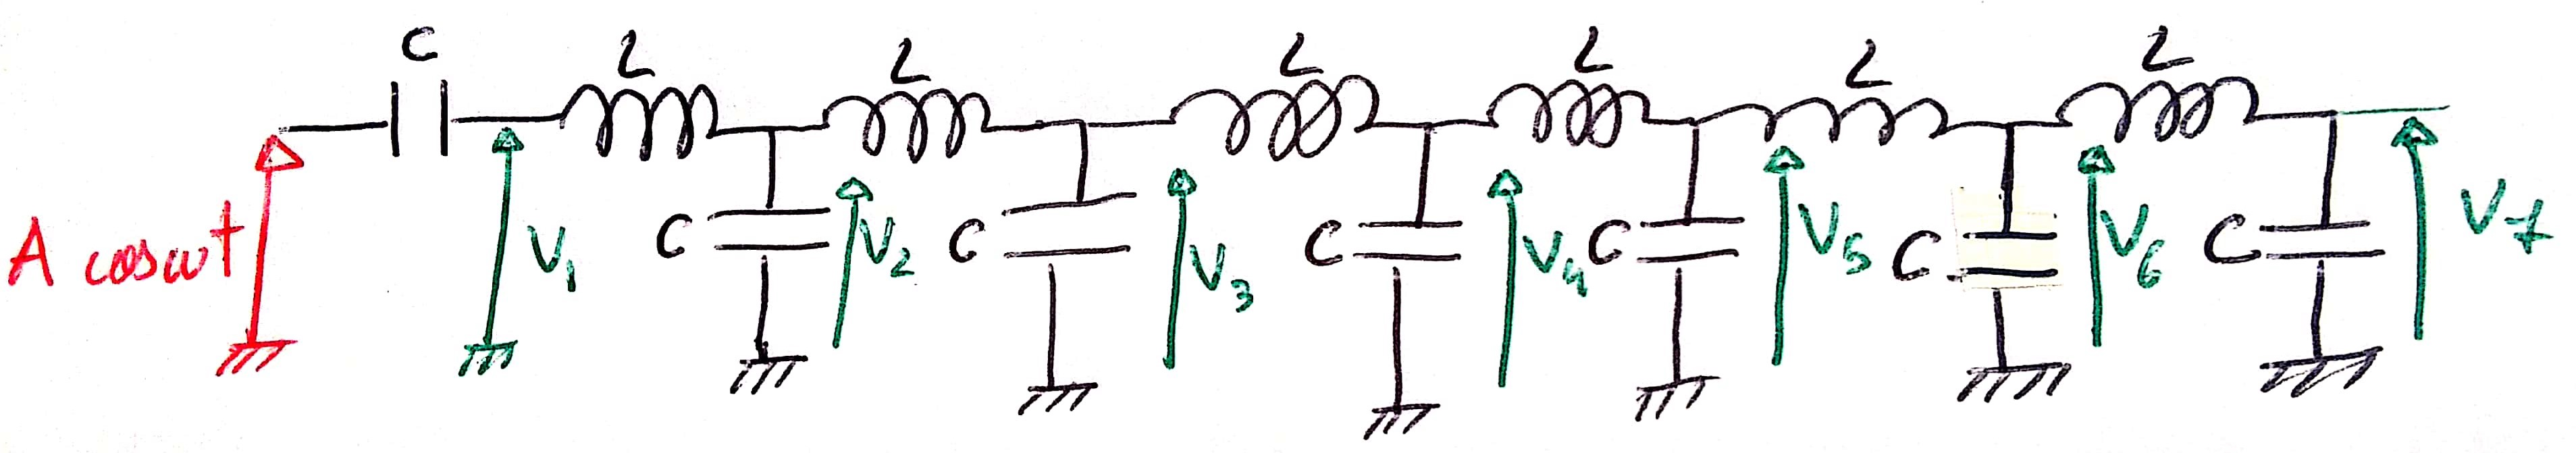
\includegraphics[width=15cm]{N_osc_couples}
\end{figure}

Il est tout d'abord possible de montrer que si on a $N$ oscillateurs alors on a $N$ modes. Pour cela on prend différentes longueur de chaînes et on regarde en faisant varier la fréquence d'un GBF délivrant une tension sinusoïdale quand est ce qu'on a résonance, ce qui est long car il faut parcourir toute la plage de fréquences propres (3$\rightarrow15$kHz environ). L'autre possibilité consiste à délivrer un créneau en entrée de période $T>5L/R$, d'acquérir la réponse indicielle et de faire alors la dérivée de la TF. On observe alors à priori un spectre sur lequel on peut relever l'amplitude et la position des $N$ modes.\\

Ceci fait il est possible de prendre la chaîne la plus longue : $N=6$ et de relever l'amplitude de chacune des 7 tensions pour chacun des modes en se plaçant à l'une des fréquences de résonance avec le GBF et en relevant la tension aux bornes de chaque condensateur. On fera attention à la phase entre le premier signal et les autres, dans le cas où il sont en opposition de phase on relèvera la seconde tension avec un signe moins. On trace ensuite pour un mode $i$ donné 
\begin{eqnarray}
V_n^i = f(n)
\end{eqnarray}
sur Régressi, avec $n$ l'indice du $n^{ieme}$ condensateur. On obtient alors une courbe semblable à une onde de tension de la forme 
\begin{eqnarray}
V^i_n(n) = A_i\sin(k_in+\phi_i)
\end{eqnarray}
On peut alors modéliser la courbe obtenue par la forme ci dessus, et relever la valeur de $k_i$ correspondant. On tracera finalement la relation de dispersion
\begin{eqnarray}
f_i = f(k_i)
\end{eqnarray}
que l'on peut comparer avec la relation de dispersion générale pour une chaine de $N$ oscillateurs LC couplés 
\begin{eqnarray}
f_i = \frac{1}{\pi\sqrt{LC}}\sin\left(\frac{i\pi}{2(N+1)}\right) = \frac{1}{\pi\sqrt{LC}}\sin\left(\frac{k_i}{2}\right) \label{dispersion}
\end{eqnarray}
où le vecteur d'onde (sans dimension) du $i^{eme}$ mode est défini comme $k_i = \frac{i\pi}{N+1}$. On vient donc de monter que l'on pouvait traiter la dynamique de $N$ oscillateurs par un formalisme ondulatoire.\\

Pour l'établissement de la relation de dispersion on pourra consulter le \textit{Cours de Berkeley tome 3 : Ondes} de \textbf{S. Crawford}. On peut cependant noter que cette relation de dispersion correspond au cas général de $N$ OH couplés qui est traité dans la leçon \textit{48 : Phénomène de résonance dans tous les domaines de la physique}.

\section{Cas de 2 oscillateurs différents}
On veut cette fois étudier ce qu'il se passe lorsque les deux oscillateurs que l'on couple sont différents. Reprenons le cas de deux LC couplés, et considérons cette fois que l'on a deux capacités $C_1$ et $C_2$ différentes, on alors 
\begin{eqnarray}
 v_1 + LC_1\frac{d^2v_1}{dt^2} +  \frac{1}{C'}(C_1v_1 -C_2v_2) = 0 &\Leftrightarrow&  \frac{d^2v_1}{dt^2} + \frac{v_1}{LC_1} +   \frac{v_1}{LC'} -\frac{C_2v_2}{LC'C_1} = 0\\
-\frac{1}{C'}(C_1v_1 -C_2v_2) + LC_2\frac{d^2v_2}{dt^2} + v_2 = 0 &\Leftrightarrow&  \frac{d^2v_2}{dt^2} + \frac{v_2}{LC_2} + \frac{v_2}{LC'} -\frac{C_1v_1}{LC'C_2}
\end{eqnarray}
que l'on peut reformuler sous forme matricielle 
\begin{eqnarray}
\begin{pmatrix}
\ddot{v}_1\\
\ddot{v}_2
\end{pmatrix}
+\begin{pmatrix}
\omega_1^2 +\omega_c^2&  -\omega_c^2k\\
-\omega_c^2/k & \omega_2^2+ \omega_c^2
\end{pmatrix}
\begin{pmatrix}
v_1\\
v_2
\end{pmatrix} = \vec{0}
\end{eqnarray}
où on a posé $\omega_i^2 = \frac{1}{LC_i}$ et $k = \frac{C_2}{C_1}$. On cherche les fréquences propres, on calcule donc les valeurs propres $\lambda$ de la matrice ci dessus 
\begin{eqnarray}
[\omega_1^2 +\omega_c^2-\lambda][\omega_2^2+\omega_c^2-\lambda] - \omega_c^4 =0\\
\lambda^2 -\lambda [\omega_1^2  +\omega_2^2 + 2\omega_c^2] + \omega_1^2 \omega_2^2 + \omega_c^2(\omega_1^2+\omega_2^2)= 0
\end{eqnarray}
on a un polynôme du second degré de déterminant 
\begin{eqnarray}
\Delta &=& [\omega_1^2  +\omega_2^2 + 2\omega_c^2]^2 - 4[\omega_1^2 \omega_2^2 + \omega_c^2(\omega_1^2+\omega_2^2)] \\
&=& \omega_1^4 + \omega_2^4 + 4\omega_c^4 - 2 \omega_1^2\omega_2^2\\
&=& (\omega_1^2-\omega_2^2)^2 + 4\omega_c^4
\end{eqnarray}
qui correspond aux valeurs propres 
\begin{eqnarray}
\lambda_{\pm} = \frac{1}{2}\left[\omega_1^2  +\omega_2^2 + 2\omega_c^2 \pm \sqrt{\Delta}\right]
\end{eqnarray}
On a donc deux pulsations propres pour notre système de deux oscillateurs couplés qui sont 
\begin{eqnarray}
\omega_{\pm} = \sqrt{\lambda_{\pm}}
\end{eqnarray}
On peut notamment vérifier que dans le cas $\omega_1=\omega_2=\omega_c = \omega_0$ on a 
\begin{eqnarray}
\Delta = 4\omega_0^4 \;\;\Longrightarrow\;\; \lambda_{\pm} = 2\omega_0^2 \pm \omega_0^2
\end{eqnarray}
on retrouve bien $\omega_s= \omega_0 = \frac{1}{\sqrt{LC}}$ et $\omega_{as} = \sqrt{3}\omega_0$ comme dans la première partie. \\

Pour ce qui est du cas général on peut tracer $\omega_{\pm} = f(\omega_1)$ pour $\omega_2$ et $\omega_c$ donnés afin d'observer ce qu'il se passe lorsque les deux oscillateurs sont différents. On a tracé $\omega_{\pm} = f(\omega_1)$ en rouge, sur la figure de gauche dans le cas d'un couplage faible : $\frac{1}{C'} = \frac{1}{10}\frac{1}{C_2}$, et sur la figure de gauche dans le cas d'un couplage plus fort $\frac{1}{C'} = \frac{1}{C_2}$. Dans les deux cas on a représenté en vert le cas où il n'y a pas de couplage entre les deux oscillateurs. Les valeurs utilisées sont $L=40$mH et $C_2$ = 0.5$\mu$F.
\begin{figure}[h]
	\centering 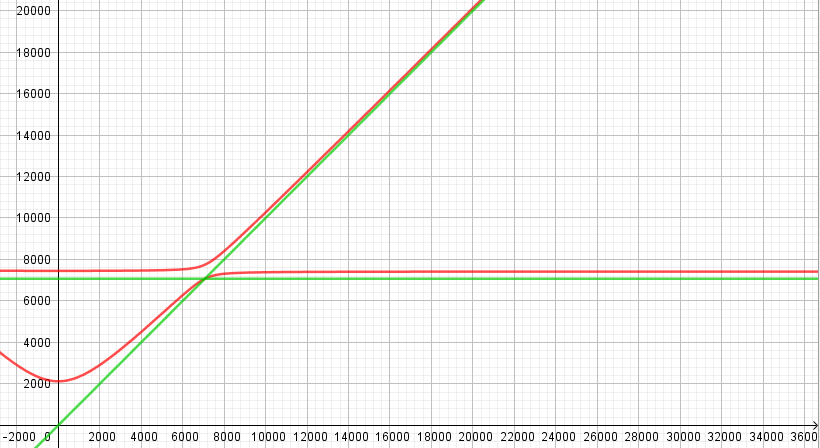
\includegraphics[width=8.5cm]{couplage_faible} 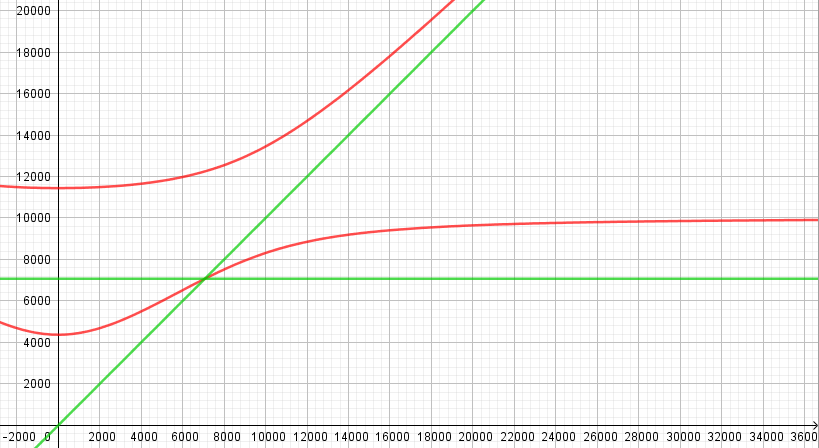
\includegraphics[width=8.5cm]{couplage_fort}
	\caption{Tracé de $\omega_{\pm} = f(\omega_1)$ en rouge avec couplage et en vert sans couplage. On a pris $C_2$ = 0,5$\mu$F et $L$ = 36mH. A gauche on a le cas couplage faible et à droite le cas couplage fort.}
\end{figure}

On constate que c'est lorsque les deux oscillateurs sont similaires (point $\omega_1\simeq 7000$ rad.s$^{-1}$) que l'effet du couplage est le plus fort.\\

On a a la possibilité de refaire cette courbe expérimentalement en prenant une boîte à décade en guise de capacité pour l'un des circuits, et en faisant ainsi une mesure des deux fréquences propres pour un éventail de valeurs de $C_1$ allant du pF au $\mu$F, et donc de $\omega_1$ allant de 1500 rad.s$^{-1}$ à 5.10$^6$ rad.s$^{-1}$.

\end{document}